\chapter{Background}

\section{Automatic speech recognition}
\label{subsec:ASR}
The goal of the automatic speech recognition(ASR) is to search the most likely sentence($\hat{W}$) in a language $L$ given acoustic observation $O$ \cite{Jurafsky:2009:SLP:1214993}. ASR has been applied in many applications and domains, for example: automatic closed captioning for hearing-disabled persons \cite{Patel2010}, taking notes of conversations between doctors and patients \cite{Klann2008}, automatic closed captioning TV broadcasts \cite{Woodland2015}, and many more.

Observation $O$ can be seen as a sequence of sliced acoustic signal. Each successive index represents the consecutive slices of acoustic input.
\begin{equation}
O=o_{1},o_{2},o_{3},...,o_{t}
\end{equation} 
A sentence is composed of a sequence of words.
\begin{equation}
W = w_{1},w_{2},w_{3},...,w_{n}
\end{equation}


Thus, an automatic speech recognition can be formalized as following:
\begin{equation}
\label{asrEq}
\hat{W} = \textrm{argmax}_{W \in L} P(W|O)
\end{equation}

Applying the bayes rule to the equation \ref{asrEq} produces the equation bellow. Because observations $O$ do not change for every possible sentence, we can assume $P(O)$ as a constant and ignore it.
\begin{align}
\hat{W} & = \textrm{argmax}_{W \in L} \textrm{ } \frac{P(O|W) \times P(W)}{P(O)} \\
	& = \textrm{argmax}_{W \in L} \textrm{ } P(O|W) \times P(W)
\end{align}
where $\hat{W}$ is the most likely sentence, $P(W)$ is the prior probability of sentence $W$ computed by the language model, and $P(O|W)$ is the observation likelihood calculated by the acoustic model. This internship mainly focuses on the acoustic model. We will discuss the language and acoustic model more in the next subsection. 



\section{N-Gram Language model}


A language model is a statistical model which computes the probability of word sequence. One of the most common language model is N-gram language model, which we leverage in this internship. The foundation mathematics of N-Gram language model was proposed by Markov in 1913. Then, Shannon re-introduced N-gram to compute the likelihoods of English word sequences \cite{Shannon:2001:MTC:584091.584093}. N-gram language model has been applied in many applications, such as: speech recognition\cite{Woodland2015}, handwriting recognition \cite{Poznanski2016}, as well as spelling correction \cite{Kukich1992}.

The goal of language model is to compute the probability ($P(w|h)$) of a word $w$ given previous word history $h$ . The way to compute this probability is by using a large corpus and count the relative frequencies. For example: to count the word $w_{1}$ given history: $w_{2}, w_{3}, ..., w_{n}$, the probability is as following:
\begin{equation}
P(w_{1}|w_{2}w_{3}...w_{n})= \frac{C(w_{1}w_{2}w_{3}...w_{n})}{C(w_{2}w_{3}...w_{n})}
\end{equation}

Because we can create infinitely possible sentences, it is more efficient to compute probability by applying the chain rule of probability. 
\begin{align*}
P(w_{1}^{n}) & =P(w_{1})P(w_{2}|w_{1})P(w_{3}|w_{1}^{2})...P(w_{n}|w_{1}^{n-1}) \\
& = \Pi_{k=1}^{n} P(w_{k}|w_{1}^{k-1})
\end{align*}

However, the probability of a word given preceding words is infeasible to be computed. Instead of computing the entire preceding history, N-gram only approximates the probability with last few words. For example: the bigram LM approximates the probability of a word given history by the probability of a word given the last word only $P(w_{n}|w_{n-1})$.  This approximation(or assumption) is called Markov assumption.

A major problem exists in N-Gram language model. Information inside a corpus might be limited. Some word sequences probably do not exist in the corpus, but they are perfectly acceptable word sequences. If we calculate the N-Gram likelihood for these sequences, we will get zero value. The solutions to the problem are backoff and smoothing. Backoff allows the N-gram LM to use the value of lower N-Gram LM if we have zero probability in the higher N-Gram.  Smoothing is a technique to avoid  zero probability for every word sequence. If a word sequence does not exist in the corpus, the LM still produces a non-zero value even though it is small. We used Kneser-Ney smoothing \cite{KneserNey1993} which has been implemented in SRILM framework.

To evaluate the performance of a language model(LM), perplexity can be applied to the LM. The intuition behind LM is given two N-gram LM, the better model is the one which predicts test set better than the other. Lower perplexity means that the model is better. Given a language model and a test corpus, perplexity is calculated as following \cite{Bahl:1983:MLA:2053027.2053281} \cite{Klakow:2002:TCW:638078.638080}:
\begin{equation}
PP = exp(-\frac{1}{N} \sum^{N}_{i=1} \log P(w_{i}|h_{i}))
\end{equation}
where $N$ is the number of words in test corpus, $w_{i}$ is the i-th word, and $h_{i}$ is the history of word $w_{i}$.


\section{Acoustic model}
The acoustic model(AM) is commonly based on hidden markov model(HMM). Thus, before talking about the acoustic model deeply, it is better to elaborate HMM first. 


\subsubsection{Markov chain}
A weighted state finite automaton is a finite state automaton where the arc between nodes has probability how likely the path is taken. Markov chain is one kind of weighted state finite automata which the input sequence determines which state the automaton will go.

Markov chain can be defined formally as following:
\begin{itemize}
\item $Q=q_{1}q_{2}...q_{N}$ a set of states
\item  $A=
\begin{bmatrix}
a_{01}a_{02}a_{03}...a_{0n} \\
a_{11}a_{12}a_{13}...a_{1n} \\
... \\
a_{01}a_{02}a_{03}...a_{0n} \\
\end{bmatrix}
$ is a transition probability matrix where $a_{ij}$ represents the probability of moving from state $i$ to state $j$. In addition to that, the sum of outgoing probability of every state must be summed into 1. $\sum_{j=1}^{n}  a_{ij}=1$. 
\item $q_{0}$ and $q_{F}$ represent initial and final states.
\end{itemize}

\subsubsection{Hidden markov model(HMM)}
\label{HMM}
Markov chain is only usable if the event is directly observable in the world. However, we are interested in some events which are not observable or hidden for some problem. For example: acoustic event is observable, but word event is not observable in speech recognition problem. Hidden markov model fixes this problem. 

Hidden markov model is formalized as 
\begin{itemize}
\item $Q=q_{1}q_{2}...q_{n}$ is a set of states
\item  $A=
\begin{bmatrix}
a_{01}a_{02}a_{03}...a_{0n} \\
a_{11}a_{12}a_{13}...a_{1n} \\
... \\
a_{01}a_{02}a_{03}...a_{0n} \\
\end{bmatrix}$ is a transition probability matrix where $a_{ij}$ represents the probability of moving from state $i$ to state $j$ such that $\sum_{j=1}^{n}  a_{ij}=1$ for every $i$.
\item $O=o_{1}o_{2}...o_{T}$ is a sequence of $T$ observations.
\item $B=b_{i}(o_{t})$ is observation likelihoods(or emission probability) where state $i$ emits probability given observation $o_{t}$. 
\item $q_{0},q_{F}$ are initial and final states.

Hidden markov model employs two assumptions:
\begin{enumerate}
\item Markov assumption. The state is only dependent to the previous state.
\begin{equation}
P(q_{i}|q_{1}q_{2}...q_{i-1}) = P(q_{i}|q_{i-1})
\end{equation}
\item Output independence assumption. Output observation $o_{i}$ is only dependent with the state $q_{i}$ which produces $o_{t}$ and independent with other states and other observations.
\begin{equation}
P(o_{i}|o_{1}o_{2}...o_{i}..o_{T}q_{1}q_{2}...q_{i}..q_{N}) = P(o_{i}|q_{i})
\end{equation}

\end{enumerate}

\end{itemize}  

\subsubsection{Applying HMM to acoustic model}
In section \ref{HMM}, HMM is explained. Now, it is time to apply HMM on acoustic model. 
\begin{enumerate}
\item States \\
A state in acoustic model can represent a word, a phone, or a sub phone depending on the problem we are trying to solve. For the digit recognition problem, a state represents a sound of one number. A sequence of phone can be represented as a word string. Hence, for more complicated task, like recognizing TV broadcast, it is better to make a state representing a phone or even a sub phone. A sound of a phone is usually influenced by the preceding and successive phone. Therefore, we use three HMM states(for each phone) which capture beginning, middle, and  end of the phone. The sub phone state is commonly called as a senone.

\begin{figure}[H]
\caption{A triphone HMM model consisting of three emitting states(beginning(S0), middle(S1), and end(S2) of a phone), a transition matrix $A$, and emission probability(observation likelihood) $B$ \cite{SiliconAM}}

\includegraphics[scale=0.6]{tiphone}
\centering
\end{figure}

\item Transition matrix \\
The transition matrix in speech recognition is the probability of moving from the current sub phone state to the successive sub phone state. Unlike HMM, Speech recognition HMM does not allow arbitrary transition because of the sequential nature of language and speech. A state can go to itself or to the next states, but it can not go back to the preceding state. This kind of left-to-right constrained HMM is called Bakis network.

\item Observation \\
The observation is a sequence of acoustic feature vector. The acoustic input is divided into small chunks and converted into a feature vector.
%Acoustic feature vector is a 39-dimension which is generated based on Mel-frequency cepstral coefficient(MFCC). Each observation is a slice of 10 milliseconds audio. For one second audio, there will be 100 acoustic feature vectors where each vector has 39 features.

\item Observation likelihood \\
Observation likelihood is the probability of a feature vector which is generated by a sub phone state. 

\end{enumerate}


\section{Deep learning for acoustic model}
For our acoustic model, we used deep neural network(DNN) HMM. Beside DNN HMM, there exists gaussian mixture model(GMM) HMM. However, DNN HMM has been proven to outperform GMM DNN in practice \cite{Peddinti2015ATD}. Hence, we only discuss DNN in this report.

\subsubsection{Feedforward neural network}
Feedforward neural network(or sometimes called multilayer perceptron(MLP)) is one kind of neural network. MLP approximates function $f'(\mathbf{x})=\mathbf{y}$. MLP can be represented as $f(\mathbf{x};\mathbf{\theta})=\mathbf{y}$ and learn parameters $\mathbf{\theta}$ which maximizes function approximations. 

Perceptron is a kind of artificial neuron developed in 1960 by Frank Rosenblatt \cite{Rosenblatt1960}. A perceptron receives several inputs($x_{1}, x_{2}, ..., x_{n}$), does weighted sum $\sum_{i} x_{i}w_{i}$, and is thresholded by bias $b$ to make a decision: zero or one.
 
\begin{equation}
output = 
\begin{cases}
0 , \textrm{if } \sum_{i} x_{i}w_{i} + b \leq 0 \\
1, \textrm{if } \sum_{i} x_{i}w_{i} + b > 0
\end{cases}
\end{equation}

\begin{figure}
\label{tdnnArchitecture}
\caption{A perceptron}
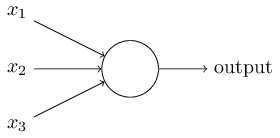
\includegraphics[scale=0.6]{perceptron}
\centering
\end{figure}

A perceptron is too simple to capture non linear pattern. Therefore, the perceptron is modified by applying an activation function into weighted sum. There are several common activation functions, such as: 
\begin{enumerate}
\item Sigmoid
\begin{equation}
a(x) = \frac{1}{1 + e ^{-x}}
\end{equation} 

\item Rectified linear unit(relu)
\begin{equation}
a(x) = max(0,x)
\end{equation} 


\item Softmax
\begin{equation}
a(x) = \frac{e^{x}}{\sum_{i} e^{x_{i}}}
\end{equation} 

\end{enumerate}

In addition to activation function, we need to make neuron to capture more complex features by stacking many neurons together. This network is called a feed forward multi layer perceptron. This neural network does not have connections between units which form a cycle. It is also called feedforward because the input values are propagated forward to output. The neural network receives inputs, does weighted sum, and applies activation function. The output of the units in one layer is propagated to the units in the next layer until reaching output layer. 

\begin{figure}[H]
\caption{Multi layer perceptron}
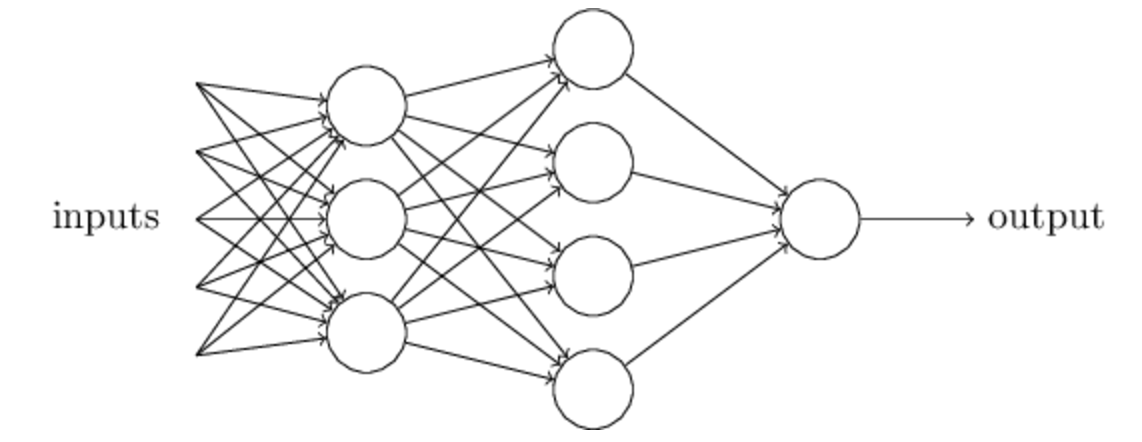
\includegraphics[scale=0.6]{mlp}
\centering
\end{figure}

\subsubsection{Time delay neural network(TDNN)}
To model a temporal sequence neural network, like the speech recognition problem, the model must have the following properties: it must have multiple layers to learn complex non linear decision surface, represents relationships between events in time, invariant under translation in time, and does not require precise temporal alignment. From all of these properties, time delay neural network(TDNN) qualifies to model a temporal sequence neural network.

There exist two ways to capture long temporal contexts:
\begin{enumerate}
\item Feature representation which present the information of long temporal contexts. The examples of the feature representation are TRAPs\cite{Hermansky99temporalpatterns}, multiscale spectro-temporal modulations representation\cite{Mesgarani04speechdiscrimination}, deep scattering spectrum representation\cite{Anden2014}, and modulation frequency feature representations\cite{Thomas2009}. These feature representations can use the standard feed forward deep neural network to model the temporal sequence neural network.

\item Acoustic model which can learn long temporal contexts and is trained on short-term feature representations. Recurrent neural network(RNN) \cite{1402.1128} and time delay neural network \cite{Waibel:1990:PRU:108235.108263} are two state-of-the-art acoustic models which are suitable to model this acoustic model. 
\end{enumerate}

Peddinti et al showed that TDNN performs better than RNN in term of parallelization during training\cite{Peddinti2015ATD}. Due to recurrent connections in RNN, RNN is not able to fully utilize parallelization in GPU(general processing unit) the same extent as TDNN. In addition, TDNN has been proven to have lower word error rate compared to RNN\cite{Peddinti2015ATD}. Thus, we will focus more on TDNN and trained acoustic models with TDNN in this internship.

Time delay neural network(TDNN) was first proposed by Waibel et al in 1990\cite{Waibel:1990:PRU:108235.108263}.TDNN is suitable to model long term temporal relationship within the range of $N$ delays in short term speech features; for example: MFCC feature representations. %todo explain more TDNN here

%The acoustic feature is called short term feature because it is an MFCC feature vector generated from a slice of 10 milliseconds acoustic input. 

\begin{figure}

\caption{An example of a TDNN architecture. \cite{Peddinti2015ATD}}
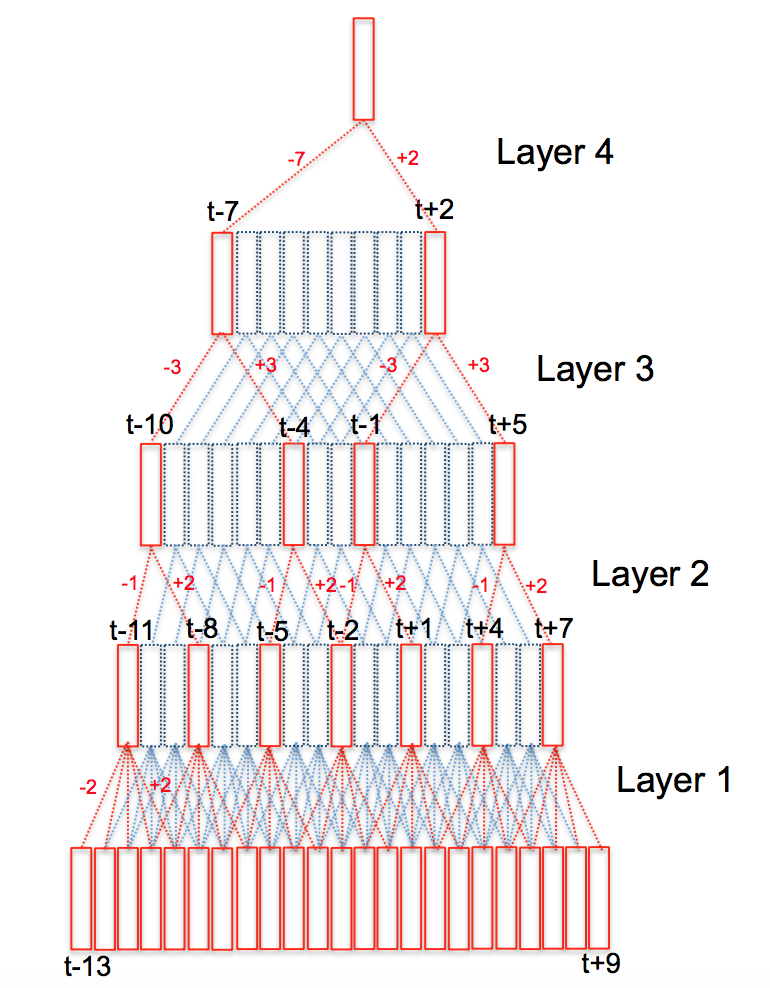
\includegraphics[scale=0.6]{tdnnArchitecture}
\label{tdnnArchitecture}
\centering
\end{figure}


%To learn sequential inputs, TDNN must learn sequence of cues. Hence, Waibel et al introduced a time delay $D_{1}$ to $D_{N}$ to learn long term temporal dependencies. The input feature vector is 40 dimensional MFCC feature vector. Figure \ref{tdnnArchitecture} shows the TDNN architecture. The input layer receives 4 delays($N=4$), i.e. $\{t-2, t-1, t, t+1, t+2\}$. Therefore, each unit has 200 weights($5 \times 40$) from input layer. The next layer(hidden layer 1) receives delay from $t-1$ through $t+2$. The higher layer will receive wider temporal contexts compared to the lower layers. For example, the final layer receives inputs which are time delay  from $t-7$ through $t+2$ context. 

TDNN is basically a feedforward neural network. Learning procedure which we used is backpropagation. There are two passes procedure in the backpropagation. The first pass is forward pass where the neural network receives input, does weighted sum, and applies activation function. The output values from the first layer is forward propagated until reaching the output layer. Then, square error is calculated between the expected value and the output of neural network. The second pass is backward pass where the derived square error value is propagated backward to update weights. 

Typical TDNN computes all hidden activation in each layer. Figure \ref{tdnnArchitecture} demonstrates an architecture of TDNN. TDNN receives acoustic inputs with some delays to the left and right contexts(before and after time $t$). Usually, the input context is asymmetric, i.e: more time context to the left than right. The main reasons are to reduce the latency of online decoding and improve word error rate. Each layer splice together contiguous temporal windows within a time range; for example: the third layer splices the frames within range $[t-3, t+3]$ in the figure  \ref{tdnnArchitecture}. Furthermore, TDNN applies wider splice when going to higher layers in the networks as shown in the figure \ref{tdnnArchitecture}. The reason is we force the higher layer to learn wider temporal contexts.

Training a TDNN is still time consuming. The standard TDNN computes all hidden activation in each layer. Consequently, the training time of TDNN is approximately ten times compared to the standard DNN.  Peddinti et al found that there exist large overlaps between input contexts at neighboring time steps; thus, they proposed subsampling \cite{Peddinti2015ATD}. The technique generally only splice no more than two temporal contexts with gap instead of contiguous temporal windows. Figure \ref{tdnnArchitecture} illustrates the procedure of subsampling. In the standard TDNN, all hidden units(red and blue) are calculated. In contrast with subsampling technique, only red hidden units are computed. In consequence, the training time of subsampled TDNN is approximately five times faster than the standard TDNN \cite{Peddinti2015ATD}. Moreover, subsampling is able to reduce the model size. Splicing contiguous temporal contexts will require a massive number of parameters. However, subsampling only splices less temporal contexts than the typical TDNN.

\subsubsection{Hybrid acoustic model}
\label{HybridAcousticModel}
To train a TDNN or other kinds of DNN acoustic model, one needs to label each acoustic input vector. However, our initial data only have utterance level of start and end time. Even, each word does not have start and end time. Each acoustic input must be labeled with its corresponding senone in order to train a DNN-HMM acoustic model. 

GMM acoustic model can bootstrap the labeling process\cite{1406.7806}. We can train a GMM-HMM acoustic model with flat start, i.e: without previous phoneme-to-audio alignment.  Therefore, the step before training a DNN acoustic model is by training a GMM-HMM acoustic model. Then, force align the training set with the acoustic inputs to generate a sequence of senone which corresponds with the transcription in the segments. The aligned data(the acoustic input with its corresponding senone) is utilized to train a DNN acoustic model.

Training a DNN-HMM is a little bit different than the HMM as explained in \ref{subsec:ASR}. An acoustic model usually models the probability $P(o|y)$ of observation(acoustic input) $o$ given its corresponding senone $y$. Nonetheless, DNN models the probability of a senone given the observation $P(y|o)$. By applying the bayes rule, $P(o|y)$ can be obtained as the following:
\begin{equation}
P(o|y)  = \frac{P(y|o) \times P(o)}{P(y)}
\end{equation}
$P(y)$ can be obtained from distribution of a senone in the training set. By using lexicon, each word in the training set can be mapped into the corresponding senone. However, $P(o)$ is infeasible to be obtained. Luckily, the observation $o$ are fixed and can be seen as a constant. Hence, we can provide HMM with the unnormalized probability..
\begin{equation}
\frac{P(y|o) }{P(y)}
\end{equation}

Applying the hybrid approach has been introduced over 20 years ago \cite{Bourlard:1993:CSR:562393,Renals1994}. Nevertheless, it did not outperform GMM until recently. DNN reduces substantial amount of word error rate compare to GMM \cite{Dahl2011,38130}. DNN excels in improving accuracy due to more representational capacity compared to GMM \cite{1406.7806}. There are several factors why DNN outperforms GMM just recently.
\begin{itemize}
\item The amount of training dataset has increased. DNN usually works well when there exists a massive volume of training data.
\item Training DNN can be done on GPU which accelerates the execution time. 
\item We have more powerful neural network architecture recently with more number of parameters, more hidden layers(deeper network), and better initialization procedure. 
\end{itemize}

% It subsamples $t-1$ and $t+2$ time(without including $t$ and  $t+1$ time samples) in the second layer, subsamples $t-3$ and $t+3$ in the third layer, and subsamples $t-7$ and $t+2$ in the final layer. 

% advantage of TDNN is it can reduce computational time and model size.

%\section{Lexicon}

